\documentclass[10pt,letterpaper]{article}
\usepackage[margin=0.72in]{geometry}
\usepackage[T1]{fontenc}
\usepackage[utf8]{inputenc}
\usepackage{lmodern,microtype,graphicx,booktabs,tabularx,longtable,amsmath}
\usepackage[table]{xcolor}
\usepackage{enumitem,fancyhdr}
\usepackage[colorlinks=true,linkcolor=blue!45!black,urlcolor=blue!45!black,citecolor=blue!45!black]{hyperref}
\hypersetup{pdftitle={PokerLab: Research Strategies and Benchmarks},pdfauthor={PokerLab / Sadegh Nouri}}
\definecolor{ink}{HTML}{21344C}
\definecolor{accent}{HTML}{147D92}
\pagestyle{fancy}\fancyhf{}\fancyhead[L]{\small\textcolor{ink}{PokerLab / research strategies}}
\fancyhead[R]{\small 12 November 2026}\fancyfoot[R]{\thepage}
\setlength{\headheight}{14pt}\setlength{\parindent}{0pt}\setlength{\parskip}{6pt}
\setlist[itemize]{nosep,leftmargin=*}
\setlength{\tabcolsep}{5pt}\renewcommand{\arraystretch}{1.12}
\begin{document}
\thispagestyle{empty}
{\small\textcolor{accent}{POKERLAB\quad /\quad EXPERIMENTAL METHODS\quad /\quad 2026-11-12}}

{\LARGE\bfseries\textcolor{ink}{From poker papers to selectable agents}}

{\large Literature, six working research options, and a reproducible evaluation}

\textbf{Result.} Six regret-minimization methods are now selectable alongside the
original 80 policies. They work correctly in a small imperfect-information
game. Their current Hold'em adaptations, however, all underperform S55 against
the fixed opponent field. \textbf{Keep S55 as the default.} These results do not
evaluate or refute the original papers' full-scale systems.

\textbf{Deliverables.} Eighteen primary-source research leads with a dated
citation snapshot; CFR, external-sampling MCCFR, CFR+, DCFR, PCFR+ and PDCFR+
solvers; frozen policies; a Mac GUI selector and heads-up practice mode;
192,500 final hands and an additional retained 192,500-hand initial screen.
The repository is \url{https://github.com/msnouri/PokerLab}.

\section*{The result that determines the default}
The final field test contains 140,000 heads-up hands: seven candidates, four
fixed opponents, and 2,500 shuffled deals per matchup, each replayed in both
seats. Each candidate therefore has 20,000 field hands but \emph{10,000
independent deal units}. The score pools the four equally represented styles.

\begin{center}\small\begin{tabular}{lrr}
\toprule
Option & Mean [95\% CI], bb/100 & Paired change vs S55 [95\% CI] \\
\midrule
S55 S55 baseline & +11.35 [+0.59, +22.12] & -- \\
R01 CFR & -20.66 [-33.55, -7.76] & -32.01 [-43.81, -20.21] \\
R02 MCCFR & -22.15 [-36.30, -8.00] & -33.50 [-46.65, -20.35] \\
R03 CFR+ & -14.58 [-27.48, -1.67] & -25.93 [-37.80, -14.06] \\
R04 DCFR & -16.59 [-29.07, -4.10] & -27.94 [-39.47, -16.41] \\
R05 PCFR+ & -15.25 [-27.77, -2.72] & -26.60 [-38.10, -15.10] \\
R06 PDCFR+ & -13.14 [-25.52, -0.76] & -24.49 [-35.94, -13.04] \\
\bottomrule
\end{tabular}
\end{center}

All six paired differences from S55 are negative. Their two-sided paired
tests remain significant after Holm adjustment for six comparisons (all
adjusted $p<0.00004$). Confidence intervals in the table are ordinary marginal
95\% intervals; they are not simultaneous intervals. R06 has the highest
research-option point estimate, but the experiment does not establish that
R06 beats the other research options.

\begin{center}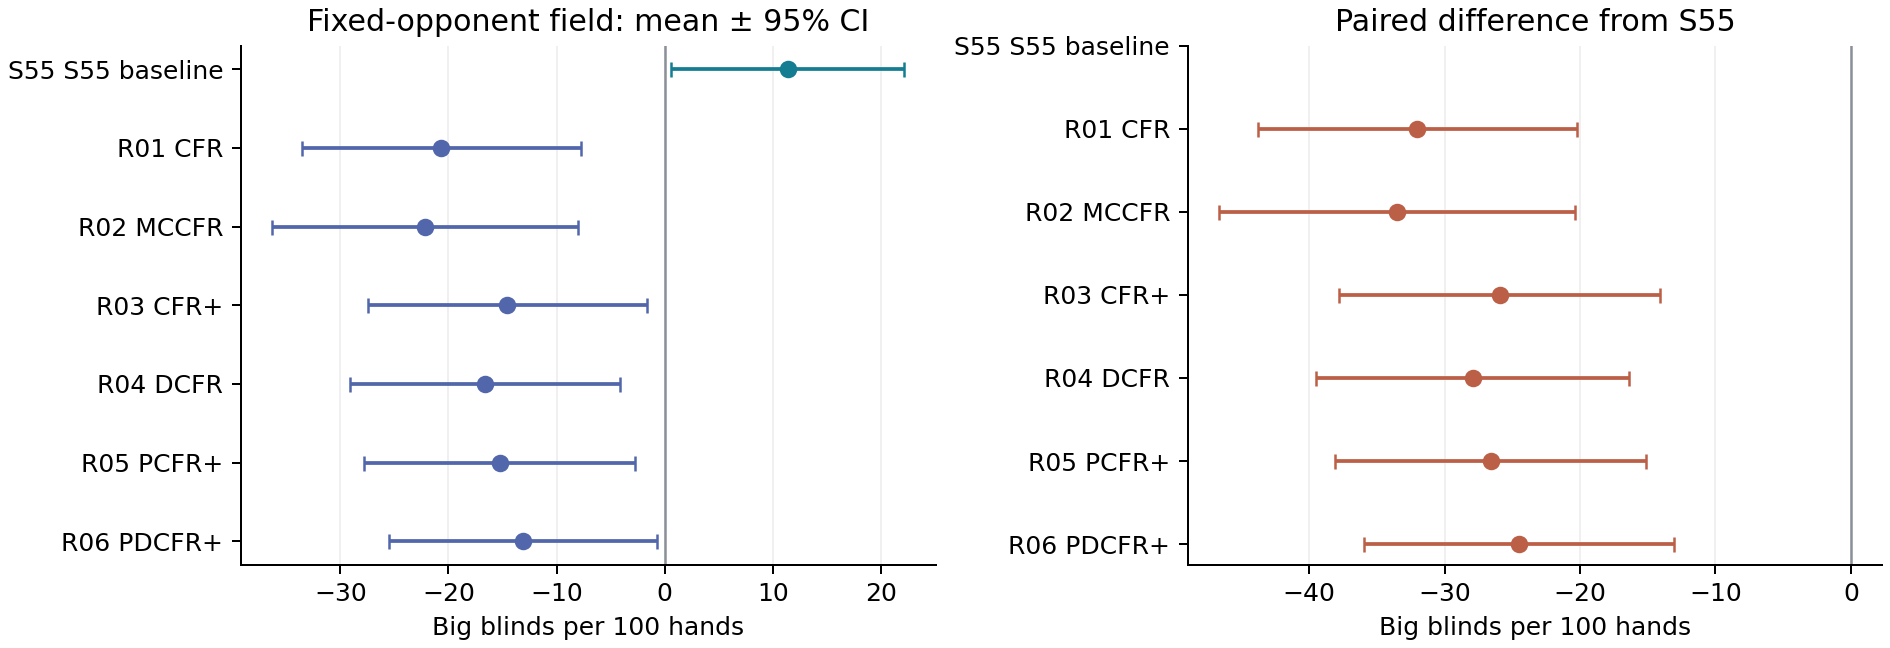
\includegraphics[width=\linewidth]{figures/field.png}\end{center}

\textbf{Interpretation.} The strongest papers describe ways to train or search
for strategies, rather than a universal list of winning moves. A good solver
cannot compensate for an inaccurate game abstraction. The next investment
should be board-dependent ranges and multi-street values, rather than changing
only the regret-update formula.

\newpage
\section*{1\quad Which papers deserve attention?}
Selection combines influence, demonstrated poker results, relevance to
no-limit Hold'em, feasible implementation and recency. Citation counts below
are OpenAlex \texttt{cited\_by\_count} snapshots from 12 November 2026, one
verified indexed work per paper. They differ from Google Scholar and can
undercount papers split across proceedings, preprints or institutional
repositories. This is a \emph{curated list}, not a global bibliometric ranking.

\begin{center}\small
\begin{tabularx}{\linewidth}{lrrX}
\toprule
Paper/system & Year & Citations & Why it matters here \\
\midrule
DeepStack \cite{deepstack} & 2017 & 882 & Heads-up continual re-solving and learned leaf values. \\
Pluribus \cite{pluribus} & 2019 & 680 & The most relevant landmark for six-player no-limit play. \\
Libratus \cite{libratus} & 2018 & 606 & Heads-up blueprint, subgame solving and self-improvement. \\
CFR \cite{cfr} & 2007 & 523 & Core self-play framework; implemented as R01. \\
NFSP \cite{nfsp} & 2016 & 443 & Neural best-response and average-policy learning. \\
Cepheus \cite{cepheus} & 2015 & 380 & Landmark CFR+ application to heads-up \emph{limit} Hold'em. \\
MCCFR \cite{mccfr} & 2009 & 207 & Sampling-based training; implemented as R02. \\
CFR+ \cite{cfr_plus} & 2014 & 164 & Practical regret matching improvements; R03. \\
\bottomrule
\end{tabularx}
\end{center}

Deep CFR \cite{deep_cfr} (2019; 105 indexed citations) addresses neural
regret approximation. DCFR \cite{dcfr} (2019; 27) and predictive CFR+
\cite{pcfr_plus} (2021; 32) supply the update rules for R04 and R05. ReBeL
\cite{rebel} (2020; 89) combines belief-state learning and search. These are
useful next readings after the basic CFR family. Counts are contextual and do
not measure which agent would win a particular match.

\subsection*{Recent work, with implementation status}
\begin{itemize}
\item \textbf{Student of Games} (2023; 62) combines search and learning across
perfect- and imperfect-information games \cite{student_games}. Reading only.
\item \textbf{Dynamic discounted CFR} (ICLR 2024; count unavailable) learns a
discount schedule \cite{ddcfr}. Reading only; no learned scheduler was trained.
An unrelated fuzzy citation match was rejected instead of reporting its count.
\item \textbf{PDCFR+} (IJCAI 2024; 7) combines weighted regret minimization
and optimistic updates \cite{pdcfr_plus}. Its tabular update is implemented as
R06 in the reduced game.
\item \textbf{SpinGPT} (2025 preprint; 2) studies an LLM approach for the
three-player Spin \& Go format \cite{spingpt}. Reading only; no weights or
training data were reproduced. Its indexed proceedings version is dated 2026.
\item \textbf{Deep (Predictive) DCFR} (AAAI 2026; 0) extends advanced updates
to neural approximations \cite{deep_pdcfr}. The publisher abstract and
metadata were reviewed; the full system was not reproduced.
\item \textbf{Parallel CFR} (2026 preprint; 10) studies a heterogeneous
CPU/GPU implementation of depth-limited solving \cite{parallel_cfr}.
Reading only; the abstract's hardware results are not Mac performance evidence.
\end{itemize}

\textbf{Reading order.} CFR $\rightarrow$ CFR+ $\rightarrow$ DCFR/PCFR+/PDCFR+
for algorithms; DeepStack and Libratus for heads-up range-aware search;
Pluribus for six-player architecture. The complete linked catalog, metadata
URLs and reusable BibTeX are in \texttt{research/}.

\newpage
\section*{2\quad What is actually implemented?}
\begin{center}\small
\begin{tabularx}{\linewidth}{llX}
\toprule
Option & Method & Update / averaging choice \\
\midrule
R01 & CFR & Alternating counterfactual regret updates; ordinary averaging. \\
R02 & External-sampling MCCFR & Sample private chance and opponent actions; expand traverser actions. \\
R03 & CFR+ & Clip cumulative regrets at zero; linear strategy weights. \\
R04 & DCFR & Positive/negative regret discounts $(\alpha,\beta)=(1.5,0)$; average exponent $\gamma=2$. \\
R05 & PCFR+ & Optimistic regret predictor; quadratic strategy weights. \\
R06 & PDCFR+ & Discounted, clipped and optimistic updates; $\alpha=2.3$, $\gamma=5$. \\
\bottomrule
\end{tabularx}
\end{center}

All six optimize a perfect-recall \textbf{one-street heads-up bucket game}:
12 independent uniform private-strength buckets, deterministic showdown
ordering, ties split, equal starting caps and one possible re-raise. Bet sizes
are quarter-, half-, full-, double- and quadruple-pot, clipped by the cap.
Six cap-to-pot depths (0.5, 1, 2, 4, 8, 16) create 36 frozen blueprints.
Full traversals receive 2,000 iterations; MCCFR receives 20,000 sampled
iterations, seed 17011. These budgets are not equal computational work.
The recorded parallel training wall time was 28.17 seconds in this environment.

For a bucket $b$, the regret-matching policy is
\[
\sigma_t(a\mid I,b)=\frac{[R_t(I,b,a)]_+}{\sum_{a'}[R_t(I,b,a')]_+},
\]
with uniform play when the denominator is zero. CFR+ clips cumulative
regrets, discounted methods reduce older regret contributions, and predictive
methods add an optimistic next-increment estimate. The implementation retains
the corresponding average policy. Update schedules were checked against the
papers and the authors' MIT reference code; source attribution is in
\texttt{research/THIRD\_PARTY\_NOTICES.md}.

\subsection*{How the frozen policy acts in Hold'em}
Only the player's own cards and public state enter inference. A shared,
deterministically seeded 48-sample random-opponent equity estimate selects a
strength bucket. Public position, pot, call cost and commitments select the
depth and betting-history node. Observed bet sizes are translated to the
nearest supported action; returned raises are translated back and bounded by
the real engine's legal raise limits. Response nodes condition on the modeled
opponent having chosen the observed bet or raise.

\textbf{Explicit S55 fallback} covers preflop, states with more than two active
players, tournaments, unknown heads-up position, unsupported histories and
off-grid depths. In six-player hands the research policy can activate after
the field falls to two active players with known public position. The GUI
displays the actual policy path, including fallback reasons. No training or
tree solving runs during a decision; policies are loaded once and looked up.

\textbf{Scope boundary.} These are actual small-game regret solvers but only
\emph{experimental Hold'em proxies}. There are no board-specific posterior
ranges, card-removal-aware joint ranges, future-street values, full-game
blueprint, neural value network, tournament ICM model or safe re-solving
guarantee. The independent uniform bucket prior is not an actual Hold'em range.
No option is named or presented as a reproduced DeepStack, Libratus or Pluribus.

\newpage
\section*{3\quad Correctness and evaluation protocol}
\subsection*{An independent known-answer check}
Standard three-card Kuhn poker has game value $u_0=-1/18$. All six methods
recover it approximately, with low exact best-response exploitability. The
test suite independently enumerates all 64 pure private-information policies
per player and checks the best-response evaluator against that enumeration.
The responder must share its action across opponent cards in each information
set; it cannot see the opponent's private card.

\begin{center}\small\begin{tabular}{lrrrr}
\toprule
Option & Iterations & $u_0$ & Exploitability & Seconds \\
\midrule
R01 & 3000 & -0.0555805 & 4.19e-04 & 0.52 \\
R02 & 30000 & -0.0555805 & 2.98e-03 & 3.00 \\
R03 & 3000 & -0.0555556 & 3.92e-05 & 0.52 \\
R04 & 3000 & -0.0555555 & 6.96e-05 & 0.56 \\
R05 & 3000 & -0.0555556 & 8.73e-10 & 0.58 \\
R06 & 3000 & -0.0555556 & 8.47e-16 & 0.60 \\
\bottomrule
\end{tabular}
\end{center}
Exploitability here is half NashConv, in game utility units. For the trained
12-bucket game at depth 4, it is also computed exactly:
\begin{center}\small\begin{tabular}{lrrr}
\toprule
Option & Iterations & Exploitability / initial pot & $u_0$ / initial pot \\
\midrule
R01 & 2000 & 0.00164 & -0.03678 \\
R02 & 20000 & 0.0413 & -0.03383 \\
R03 & 2000 & 0.000156 & -0.03648 \\
R04 & 2000 & 1.74e-05 & -0.03635 \\
R05 & 2000 & 0.000205 & -0.03645 \\
R06 & 2000 & 0.000164 & -0.03641 \\
\bottomrule
\end{tabular}
\end{center}
These numbers certify only the modeled small games. Small abstract
exploitability is not an estimate of full Hold'em exploitability or win rate.
The recorded iteration-by-iteration convergence plot is included with the
repository figures and data.

\subsection*{Hold'em test design}
\begin{itemize}
\item PokerKit enforces no-limit Texas Hold'em legality and settlement. Each
hand starts at 100 big blinds, with no rake and no cross-hand opponent learning.
\item \textbf{Field:} 140,000 hands. S08 (tight aggressive), S18 (aggressive),
S23 (value focused), S33 (bluff catching). Identical shuffled decks and both
seat assignments are used for all seven candidates. Opponents have distinct
seed blocks. These are our existing heuristic styles, not champion bots.
\item \textbf{Round robin:} 42,000 hands, all 21 candidate pairs, 1,000
duplicate deals per pair. \textbf{Six-player check:} 10,500 hands, 250 deals
per candidate repeated in all six seats versus S08, S18, S23, S33 and S78.
\item The statistical unit is one shuffled deal averaged over its two or six
seat repetitions. Approximate Student-$t$ intervals use these units. Field
differences subtract S55's outcome on the same deals. A pooled equal-opponent
field estimate is reported; between-style variation is retained in its interval.
\item Final deal seed offset is 300,000,000, separate from the initial screen.
Action draws are independent of hidden cards. Frozen blueprints are never
trained on benchmark outcomes. Raw deals, scores and hashes are retained.
\end{itemize}

\newpage
\section*{4\quad Additional playing results and response speed}
\begin{center}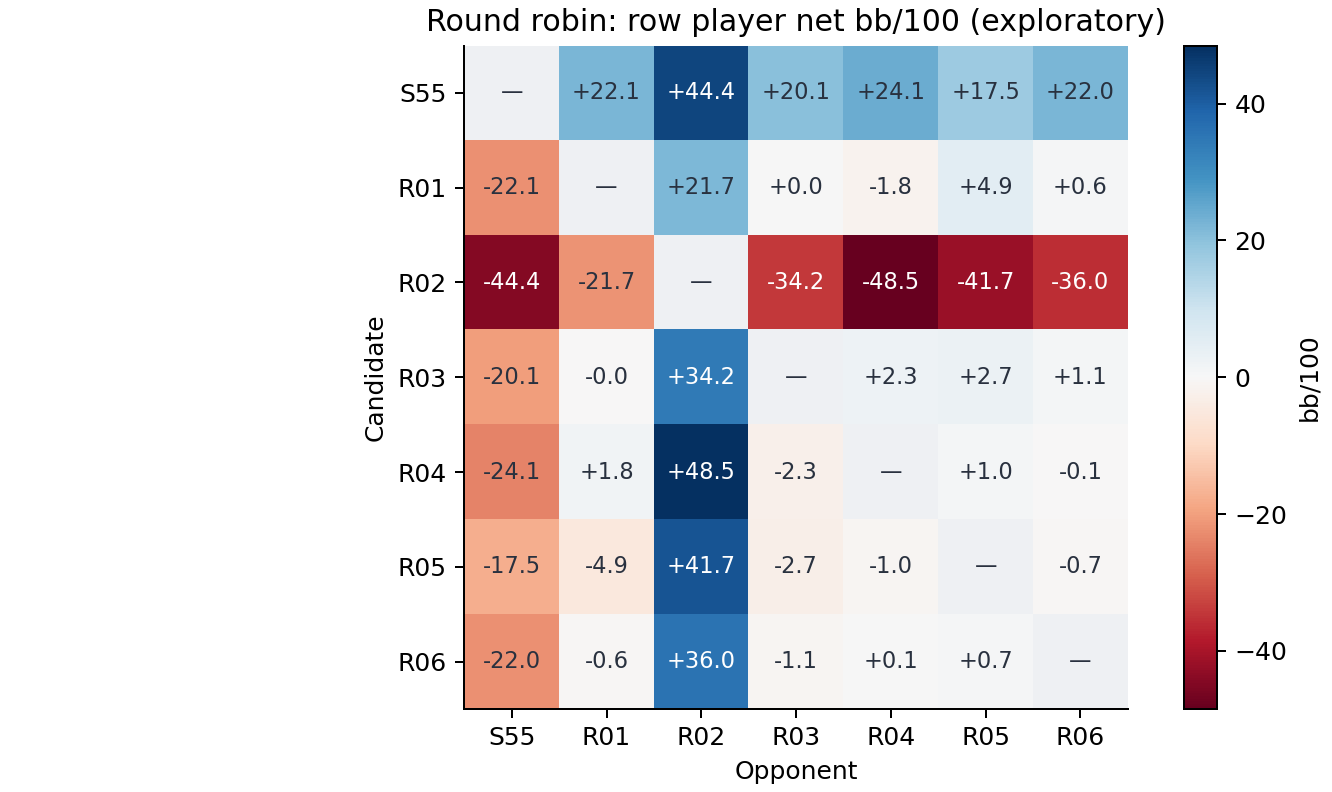
\includegraphics[width=.66\linewidth]{figures/round_robin.png}\end{center}
Every cell is a mean over 2,000 hands, or 1,000 independent duplicate deals.
Opposite cells are the same match with the sign reversed; they are not new
experiments. The diagonal was not run. Pairwise intervals are exploratory and
available in \texttt{benchmark.json}; small differences among research options
should not be treated as a reliable ranking.

\subsection*{Six-player scores and heads-up field timing}
\begin{center}\footnotesize\begin{tabular}{lrrrr}
\toprule
Option & Six-player bb/100 [95\% CI] & HU lookup & Policy p95 & Lookup p95 \\
\midrule
S55 & +0.73 [-49.20, +50.65] & 0.0\% & 0.429 & -- \\
R01 & -40.06 [-111.23, +31.11] & 26.6\% & 0.433 & 0.584 \\
R02 & -76.64 [-146.73, -6.54] & 25.9\% & 0.419 & 0.561 \\
R03 & -78.95 [-145.63, -12.27] & 26.5\% & 0.416 & 0.645 \\
R04 & -65.16 [-134.87, +4.55] & 26.2\% & 0.395 & 0.636 \\
R05 & -68.79 [-140.44, +2.86] & 26.4\% & 0.389 & 0.535 \\
R06 & -73.69 [-146.93, -0.45] & 26.2\% & 0.379 & 0.552 \\
\bottomrule
\end{tabular}
\end{center}
These estimates use only 250 independent deals per candidate and have wide
intervals. The research options use S55 while a pot is multiway and can switch
to their blueprint when only two players remain. This check does not reproduce
Pluribus or establish tournament performance.

The last two columns are milliseconds. HU lookup share is calculated from all
hero heads-up field decisions. Latency is the
largest per-opponent p95, not a pooled percentile; the last column restricts
timings to blueprint decisions. Each 250-deal work block retains up to 600
decision samples per timing category. Timings include the policy/equity call
and exclude capture, OCR, GUI painting and agent initialization. OS scheduling,
cache state and eight concurrent Python workers affect them.

The final 192,500-hand run finished in 63.85 seconds. There were zero rejected
illegal actions and zero chip-conservation errors. These are local Linux
simulation results, not native Mac end-to-end latency measurements. The existing
native Mac CI retains its Apple Vision accuracy and coverage checks and now
also runs the solver/private-information tests on ARM and Intel.

\newpage
\section*{5\quad Retained first screen and practical use}
The first adapter trained separate facing-bet roots with an unconditioned
bettor prior. All six methods lost substantially. The revision reuses learned
responses from the corresponding public betting-history nodes and expanded
the modeled bet/depth grid. The initial code, model and 192,500 raw hands are
retained under \path{poker_lab/research_results/screening_v1/}.

\begin{center}\small\begin{tabular}{lrrr}
\toprule
Option & Initial mean & Initial paired change vs S55 & Revised mean \\
\midrule
S55 & +3.86 & +0.00 & +11.35 \\
R01 & -69.51 & -73.36 & -20.66 \\
R02 & -81.99 & -85.85 & -22.15 \\
R03 & -66.13 & -69.98 & -14.58 \\
R04 & -65.74 & -69.59 & -16.59 \\
R05 & -66.17 & -70.02 & -15.25 \\
R06 & -65.83 & -69.68 & -13.14 \\
\bottomrule
\end{tabular}
\end{center}
All figures above are bb/100. The revised run used fresh deals, so differences
between versions are descriptive, not paired effects. Only one adapter
revision was evaluated; the unfavorable initial screen remains visible. The
revision improved point estimates but still failed to beat the existing
baseline. No option was promoted on the strength of a selectively reported run.

\subsection*{Selecting an option on Mac}
Launch Vision Studio normally and choose \textbf{Open agent lab}, or run
\texttt{python -m desktop --classic}. In the practice workbench, choose
\textbf{Heads-up / two players} and select R01--R06 in the strategy menu.
S55 remains selected by default. Recommendations identify whether a paper
blueprint or S55 fallback actually made the decision. The JSON bot also accepts
\texttt{--strategy R06}. The original 80-policy experiment remains unchanged.

\subsection*{Reproducing the work}
From a Python 3.12 environment with the repository requirements installed:
\begin{verbatim}
PYTHONPATH=poker_lab python -m pokerlab.research.train
PYTHONPATH=poker_lab python -m pokerlab.research.convergence \
  --output poker_lab/research_results/convergence.json
PYTHONPATH=poker_lab python -m pokerlab.research.benchmark \
  --pairs 2500 --round-robin-pairs 1000 --multiway-deals 250 \
  --seed-offset 300000000 --workers 8 \
  --output poker_lab/research_results
make test-research
make research-report
\end{verbatim}
Training is optional when using the checked-in frozen model. Rebuilding the
report audits all 192,500 final raw rows and independently recalculates the
confidence intervals. Seeds determine playing outcomes; timing fields and
gzip headers can change output-file hashes on rerun. The included SHA256
manifest binds the recorded output to the frozen model used here.

\subsection*{What would justify changing the default?}
First build board-dependent, action-conditioned ranges and multi-street
counterfactual values, and check that abstraction choices preserve decision
quality. Then test against stronger pinned external agents and on untouched
deals, using duplicate matches and variance reduction where appropriate.
Evaluate six-player and tournament play separately. A native Mac capture-to-
recommendation replay must measure the full latency budget. Until then, these
options are useful research controls, with no supported claim of being a
winning real-world poker system.

\newpage
\small
\begin{thebibliography}{99}

\bibitem{deepstack} Matej Moravcik and Martin Schmid and Neil Burch and Viliam Lisy and Dustin Morrill and Nolan Bard and Trevor Davis and Kevin Waugh and Michael Johanson and Michael Bowling. \emph{DeepStack: Expert-level artificial intelligence in heads-up no-limit poker}. 2017. \url{https://doi.org/10.1126/science.aam6960}.

\bibitem{pluribus} Noam Brown and Tuomas Sandholm. \emph{Superhuman AI for multiplayer poker}. 2019. \url{https://doi.org/10.1126/science.aay2400}.

\bibitem{libratus} Noam Brown and Tuomas Sandholm. \emph{Superhuman AI for heads-up no-limit poker: Libratus beats top professionals}. 2018. \url{https://doi.org/10.1126/science.aao1733}.

\bibitem{cfr} Martin Zinkevich and Michael Johanson and Michael Bowling and Carmelo Piccione. \emph{Regret Minimization in Games with Incomplete Information}. 2007. \url{https://poker.cs.ualberta.ca/publications/NIPS07-cfr.pdf}.

\bibitem{nfsp} Johannes Heinrich and David Silver. \emph{Deep Reinforcement Learning from Self-Play in Imperfect-Information Games}. 2016. \url{https://arxiv.org/abs/1603.01121}.

\bibitem{cepheus} Michael Bowling and Neil Burch and Michael Johanson and Oskari Tammelin. \emph{Heads-up limit holdem poker is solved}. 2015. \url{https://doi.org/10.1126/science.1259433}.

\bibitem{mccfr} Marc Lanctot and Kevin Waugh and Martin Zinkevich and Michael Bowling. \emph{Monte Carlo Sampling for Regret Minimization in Extensive Games}. 2009. \url{https://papers.nips.cc/paper/2009/hash/00411460f7c92d2124a67ea0f4cb5f85-Abstract.html}.

\bibitem{cfr_plus} Oskari Tammelin. \emph{Solving Large Imperfect Information Games Using CFR+}. 2014. \url{https://arxiv.org/abs/1407.5042}.

\bibitem{deep_cfr} Noam Brown and Adam Lerer and Sam Gross and Tuomas Sandholm. \emph{Deep Counterfactual Regret Minimization}. 2019. \url{https://proceedings.mlr.press/v97/brown19b.html}.

\bibitem{rebel} Noam Brown and Anton Bakhtin and Adam K. Lerer and Qucheng Gong. \emph{Combining Deep Reinforcement Learning and Search for Imperfect-Information Games}. 2020. \url{https://arxiv.org/abs/2007.13544}.

\bibitem{student_games} Martin Schmid and Matej Moravcik and Neil Burch and Rudolf Kadlec and Josh Davidson and Kevin Waugh and Nolan Bard and Finbarr Timbers and Marc Lanctot and G. Zacharias Holland and Elnaz Davoodi and Alden Christianson and Michael Bowling. \emph{Student of Games: A unified learning algorithm for both perfect and imperfect information games}. 2023. \url{https://doi.org/10.1126/sciadv.adg3256}.

\bibitem{pcfr_plus} Gabriele Farina and Christian Kroer and Tuomas Sandholm. \emph{Faster Game Solving via Predictive Blackwell Approachability: Connecting Regret Matching and Mirror Descent}. 2021. \url{https://doi.org/10.1609/aaai.v35i6.16676}.

\bibitem{dcfr} Noam Brown and Tuomas Sandholm. \emph{Solving Imperfect-Information Games via Discounted Regret Minimization}. 2019. \url{https://doi.org/10.1609/aaai.v33i01.33011829}.

\bibitem{parallel_cfr} Boning Li and Longbo Huang. \emph{Real-Time Parallel Counterfactual Regret Minimization}. 2026. \url{https://arxiv.org/abs/2605.19928}.

\bibitem{pdcfr_plus} Hang Xu and Kai Li and Bingyun Liu and Haobo Fu and Qiang Fu and Junliang Xing and Jian Cheng. \emph{Minimizing Weighted Counterfactual Regret with Optimistic Online Mirror Descent}. 2024. \url{https://www.ijcai.org/proceedings/2024/583}.

\bibitem{spingpt} Narada Maugin and Tristan Cazenave. \emph{SpinGPT: A Large-Language-Model Approach to Playing Poker Correctly}. 2025. \url{https://arxiv.org/abs/2509.22387}.

\bibitem{deep_pdcfr} Hang Xu and Kai Li and Haobo Fu and Qiang Fu and Junliang Xing and Jian Cheng. \emph{Deep (Predictive) Discounted Counterfactual Regret Minimization}. 2026. \url{https://ojs.aaai.org/index.php/AAAI/article/view/38780}.

\bibitem{ddcfr} Hang Xu and Kai Li and Haobo Fu and Qiang Fu and Junliang Xing and Jian Cheng. \emph{Dynamic Discounted Counterfactual Regret Minimization}. 2024. \url{https://proceedings.iclr.cc/paper_files/paper/2024/hash/a89331e2ecbbd9d9618bc94717a91155-Abstract-Conference.html}.

\end{thebibliography}

\end{document}
